\emph{Dans cette partie d'Analyse, nous appellerons notre modèle d'IA \cogito{}.}

\section{Généralités}

\subsection{Architecture générale}
\label{subsection_architecture_generale}
L'architecture générale de \cogito{} est présentée sur la figure~\ref{schema_general}. Elle est composée de trois modules :
\begin{itemize}
\item l'analyseur, composé d'un \emph{RuleBook}, d'un analyseur conceptuel de base et d'un analyseur conceptuel poussé,
\item le raisonneur, qui contient un moteur de choix, et un module d'introspection,
\item et la mémoire, structurée avec une interface nommée mémoire primaire.
\end{itemize}

\begin{figure}[H] 
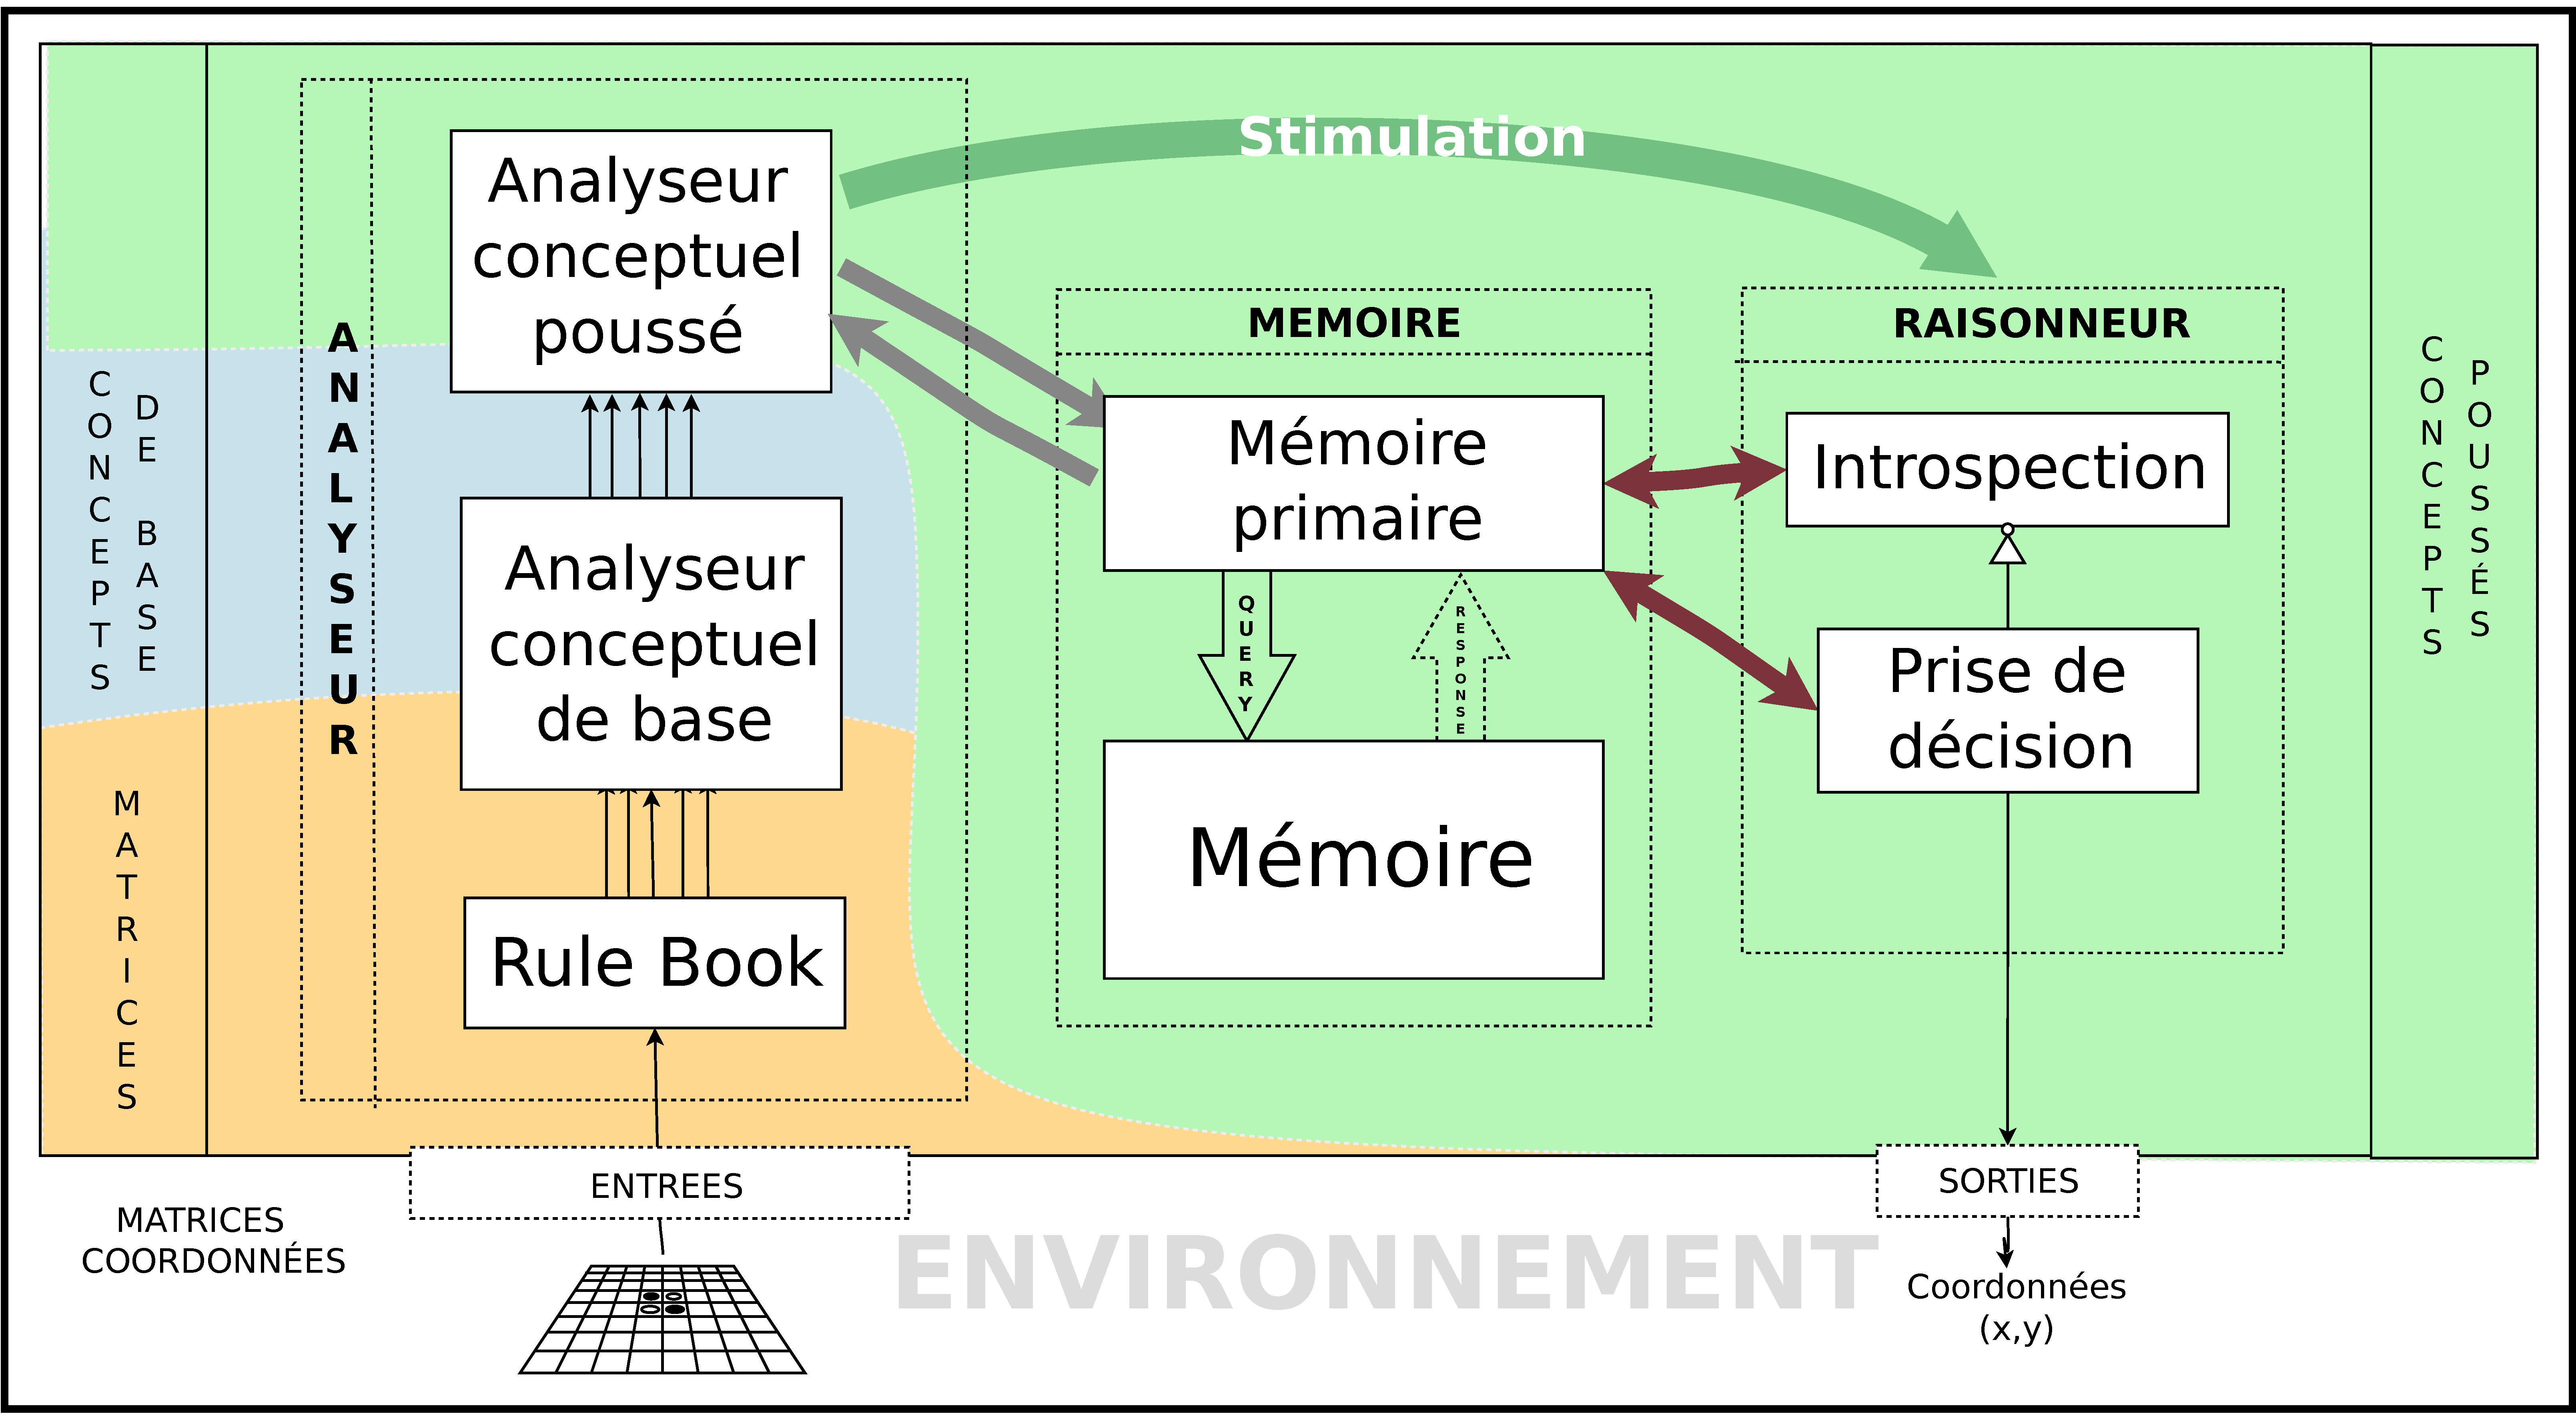
\includegraphics[width=\textwidth]{files/simplified_general_diagram} 
\caption{Schéma général de \cogito{}.} 
\label{schema_general}
\end{figure}

L'environnement est externe à l'agent, et interagit avec ce dernier via ses entrées~/~sorties.

Trois niveaux de données sont manipulés par l'IA :
\begin{itemize}
\item des données sous forme matricelle provenant de l'environnement,
\item ces mêmes données décrites dans un formalisme logique,
\item et enfin, les données précédentes associées à des formes connues, que nous appelerons concepts poussés.
\end{itemize}

\subsection{Déroulement d'un coup}
\label{deroulement_dun_coup}

\begin{figure}[p]
\centering
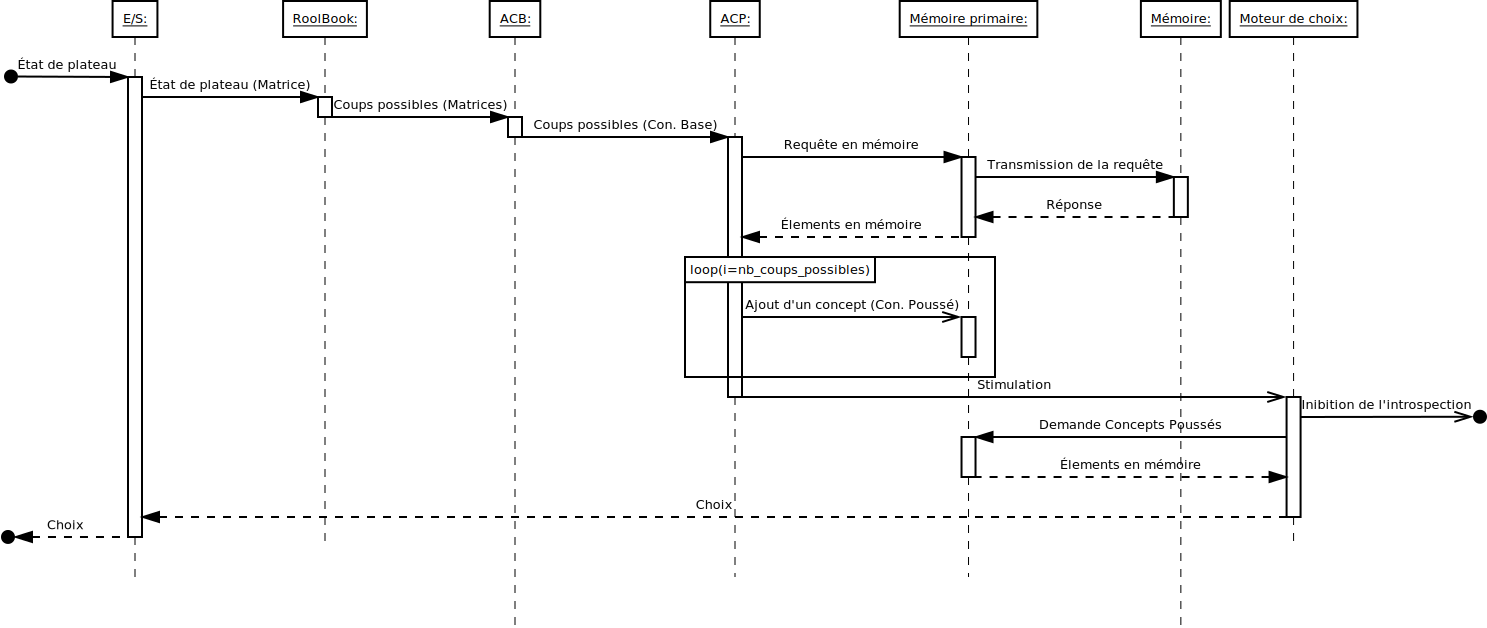
\includegraphics[width=0.9\textheight,angle=90]{files/analyse/sequence}
\caption{Diagramme de séquence sommaire de déroulement d'un coup.}
\label{diag_sequence_coup}
\end{figure}

La figure~\vref{diag_sequence_coup} décrit les interactions entres les modules de l'IA lorsque qu'un coup doit être joué.

Un plateau, décrit sous forme matricielle, est transmit par l'environnement, via un module d'\emph{E/S}\footnote{Entrée/Sortie}, au \emph{RuleBook}. Ce dernier détermine l'ensemble des coups possibles et génère l'ensemble des matrices résultantes correspondantes qu'il transmet à l'\emph{ACB}\footnote{Analyseur Conceptuel de Base}. Ce module traduit les plateaux reçus d'un format matriciel dans un formalisme logique. On obtient alors un ensemble de faits dans un format logique, pouvant être vus comme une base de faits, qui est fournie à l'\emph{ACP}\footnote{Analyseur Conceptuel Poussé}. Ce dernier interroge la mémoire pour obtenir une série de formes remarquables. L'\emph{ACP} associe à chaque plateau les formes qui peuvent y être reconnues. Une fois analysé, cet ensemble, plateaux et formes remarquables, est stocké en mémoire primaire. L'\emph{ACP} stimule ensuite le module de raisonnement qui, à partir de l'ensemble des plateaux possibles, des formes remarquables qui y sont associées et de la valuation de ces formes fournit par la mémoire, fait un choix entre les différents coups possibles. Cette décision est successivement transmise au module d'\emph{E/S} puis à l'environnement.
